\documentclass[12pt]{article}
\usepackage{url,amsmath}
\usepackage{algorithm}
\usepackage{algpseudocode}
\usepackage{graphicx}

\renewcommand{\algorithmicrequire}{\textbf{Input:}}
\renewcommand{\algorithmicensure}{\textbf{Output:}}

\setlength{\oddsidemargin}{.25in}
\setlength{\evensidemargin}{.25in}
\setlength{\textwidth}{6.25in}
\setlength{\topmargin}{-0.4in}
\setlength{\textheight}{8.5in}

\newcommand{\heading}[5]{
   \renewcommand{\thepage}{#1-\arabic{page}}
   \noindent
   \begin{center}
   \framebox{
      \vbox{
    \hbox to 5.78in { {\bf Math/Stat 310: Intro to Mathematical Statistics}
         \hfill #2 }
       \vspace{4mm}
       \hbox to 5.78in { {\Large \hfill #5  \hfill} }
       \vspace{2mm}
       \hbox to 5.78in { {\it #3 \hfill #4} }
      }
   }
   \end{center}
%   \vspace*{4mm}
}

\newcommand{\handout}[3]{\heading{#1}{#2}{Instructor:
Hyunseung Kang}{Scribe: Meenmo Kang}{Lectures #1: #3}}

\setlength{\parindent}{0in}
\setlength{\parskip}{0.1in}

\newcommand{\Var}{{\rm Var}}
\newcommand{\E}{{\rm E}}
\newcommand{\Cov}{{\rm Cov}}
\newcommand{\Corr}{{\rm Corr}}
\newcommand{\pdf}{{\rm pdf}}
\newcommand{\mgf}{{\rm MGF}}
\newcommand{\proof}{{\bf Proof. }} %% To begin a proof write \proof
\newcommand{\qed}{\mbox{}\hspace*{\fill}\nolinebreak\mbox{$\rule{0.6em}{0.6em}$}} %%to end your proof write $\qed$.
\newcommand{\ma}{{\mathcal A}}
\newcommand{\mf}{{\mathcal F}}
\newcommand{\hs}{\heartsuit}
\newcommand{\cs}{\clubsuit}
\newcommand{\noi}{\noindent}
\newtheorem{lemma}{Lemma}
\newtheorem{theorem}[lemma]{Theorem}
\newtheorem{definition}{Definition}
\newtheorem{proposition}{Proposition}
\newtheorem{remark}{Remark}

\bibliographystyle{plain}

\begin{document}
\handout{2\&3}{February 05, 2018}{Sampling Theory \& Estimation}
%Set n to the lecture number

\begin{section}{Sampling Theory}
Since we are unable to sample a whole population for research, in reality, random sampling is needed. Suppose someone is doing a research project about the average height of all students on the campus. The ideal method to investigate is to interview every single student and measure their height one by one. $\xi$ is defined by a unit of the population that contains the height information of each individual. Then, a set of the population can be expressed as $(\xi_1,\xi_2,...,\xi_n)$. For example, $\xi_\text{Tom}$ is equal to the height of Tom. When we sum up all of the elements of the set and divide that number by the number of elements, then the result is going to be population mean $$\mu=\frac{1}{N} \sum\limits_{i=1}^n (\xi_i)$$ 

This $\mu$ will be the ideal value for research, but in most cases, it is impossible to achieve such ideals. 
Nevertheless, in an effort to achieve more credible data, researchers apply a method known as $\textbf{random sampling}$. Using this method, researchers take \textbf{n} random samples from a population whose size is \textbf{N}. There is another random variable $X_i$. While sampling n random people from N total population, $X_i$ is considered as 1 if $i^\text{th}$ person was chosen. Otherwise, $X_i$ is going to be 0. So, a set of sample is denoted by ($X_1, \ldots , X_N$). \\ 

$X_i= 
\begin{cases}
1\text{\quad In case random variable $i$ was sampled}\\
0\text{\quad Otherwise}
\end{cases}$\\ \newline

The probability density function of joint distribution, ($X_1, \ldots , X_N$) is $\frac{1}{\binom{N}{n}}$ since \textbf{N} total options can be selected, and \textbf{n} are actually sampled out of \textbf{N}. So, there are $\binom{N}{n}$ possible cases that can happen. \\ 

Assuming one unit was already chosen, we can consider the marginal probability. So, what we only need to consider is the residual fraction \textbf{n-1} samples out of \textbf{N-1}. All possible combinations to account for the denominator are same as $\binom{N}{n}$. However, on the numerator, we should subtract 1 from each \textbf{N} and \textbf{n}, as $X_i$ is excluded for consideration. Mathematically, it can be explained as below. 

$P[X_i=1] = \frac{\binom{N-1}{n-1}}{\binom{N}{n}} = \frac{(N-1)!}{(n-1)!(N-1-(n-1))!} \cdot \frac{1}{\frac{N!}{n!(N-n)!}} = \frac{(N-1)!}{(n-1)!(N-n)!} \cdot \frac{n!(N-n)!}{N!} = \frac{n}{N}$ \\

There is another way to approach $P[X_i = 1]$. Out of N total population, suppose one unit is going to be sampled. Its probability is $1-\frac{N-1}{N}$. When sampling two, it will be $1-\frac{N-1}{N} \cdot \frac{N-2}{N-1}$. That implies that sampling n out of N is $1-\frac{N-1}{N} \cdot \frac{N-2}{N-1} \ldots \frac{N-n}{N-(n-1)} = \frac{n}{N}$. \\ 

Expectation and variance of $x_i$ are quite similar with those of Bernoulli distribution, defined as $E[x_i]=\frac{n}{N}, var[x_i]=\frac{n}{N} (1- \frac{n}{N})$ respectively. However, they are dependent on each other, so we do not refer them as Bernoulli. \\

$Cov(x_i,x_j) \neq 0$ proves dependency. According to the covariance formula, \\
$Cov[x_i,x_j] = E[x_ix_j]-E[x_i]E[x_j]$. The latter part is simply the product of the expectations, which is $(\frac{n}{N})^2$. And $E[x_ix_j] = \sum\limits_{k=1}^N \sum\limits_{l=1}^N P[X_i=1 \, \text{and} \, X_j=1]$ meaning $i$th and $j$th cards are chosen at the same time. However, we sample one at a time, not all at once. This means that $i$th ($j$th) card must be picked prior to $j$th ($i$th) card. So, the equation can be expressed as a conditional probability like $P[x_i=1 \, | \, x_j=1] \times P[x_j=1]$. At first, probability of picking up $x_i$ or $x_j$ is $\frac{2}{52}$. Given one of them being selected, the probability that the other one being picked, $P[x_i = 1 \, | \, x_j=1]$ in mathematical notation, will be $\frac{1}{51}$ excluding the card already removed from the deck. Hence, $E[x_ix_j] = \frac{2 \cdot 1}{52 \cdot 51}$ \\ 

This process can also be visualized through the drawing below. For example, suppose we pick two cards randomly from a deck of 52 cards, and we want to know the probability that Ace of Diamonds and Ace of Spades are picked at the same time. For the first pick, either the Ace of Diamonds or that of the Spades should be picked out of 52 cards, and then another card should be drawn from 51 cards. So, there are two pairs out of $52 \times 51$ times, $\frac{2 \cdot 1}{52 \cdot 51}$ as we can see on the picture below.

$$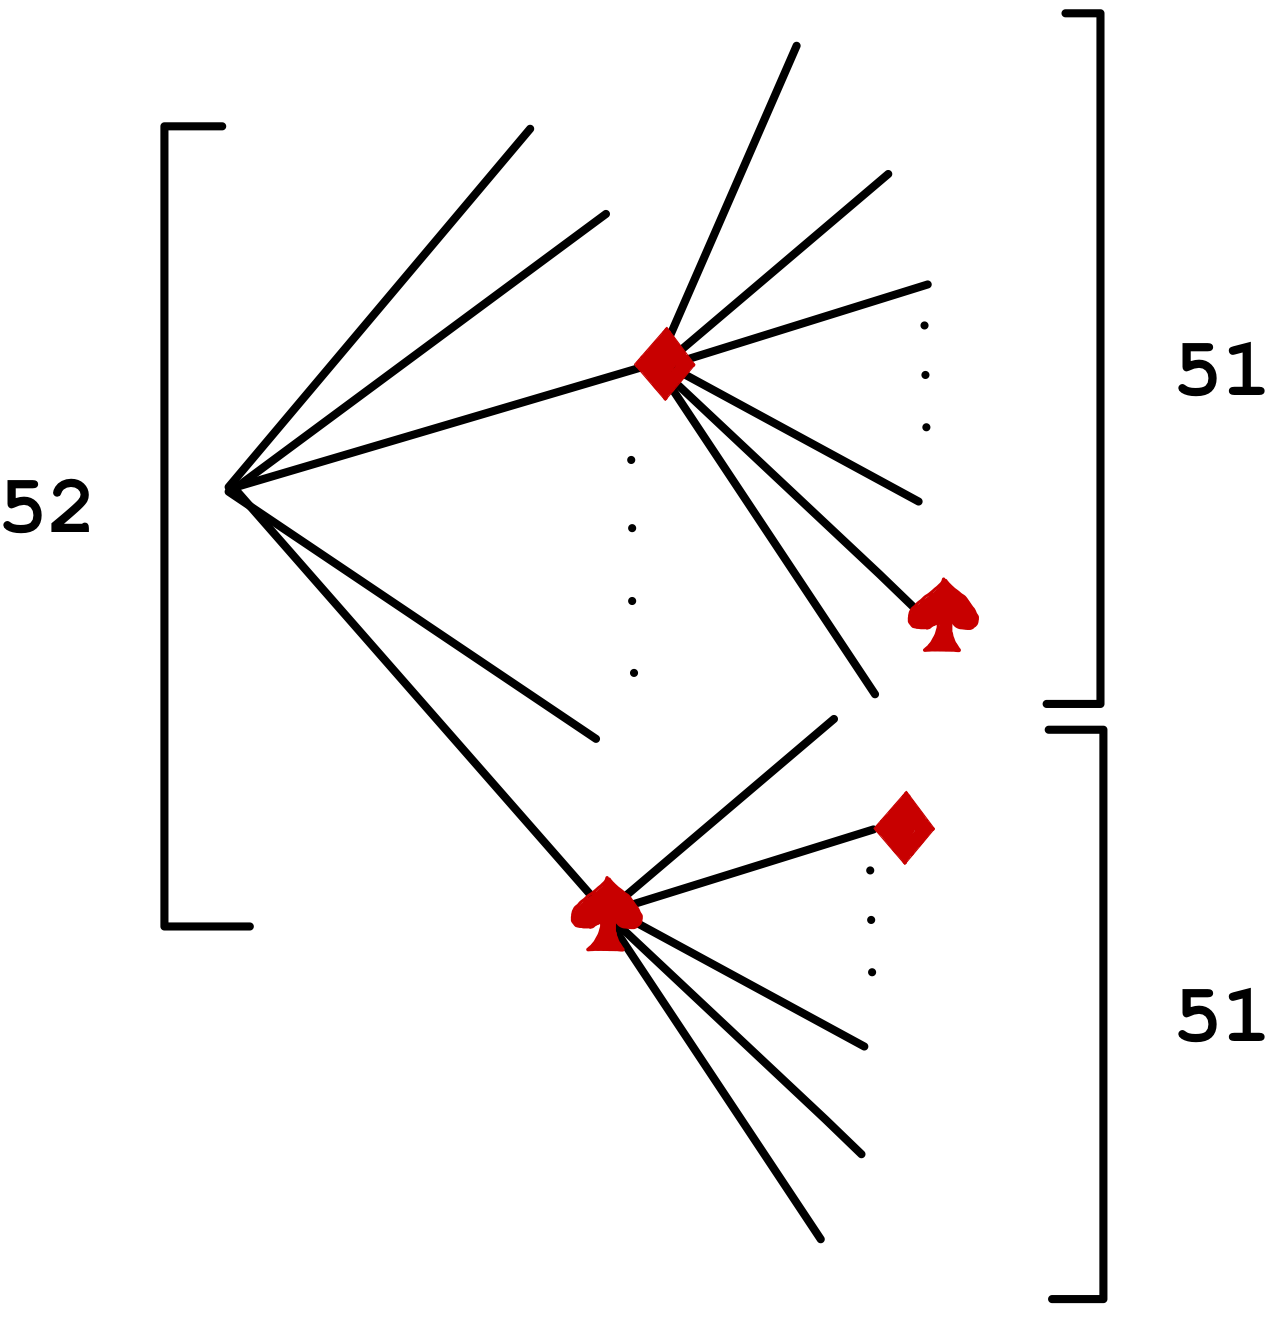
\includegraphics[height=5cm, width=5cm]{tree.png}$$

Returning to the covariance, in the end, covariance of $x_i,x_j$ becomes $\frac{n(n-1)}{N(N-1)} - (\frac{n}{N})^2$. Intuitively, what we could find from this is, firstly, that $x_i,x_j$ are negatively correlated due to $\frac{n(n-1)}{N(N-1)} < (\frac{n}{N})^2$. Secondly, as \textbf{N}, total number of sample, becomes negative, while \textbf{n} remains fixed, the covariance converges to zero. \\

\section{Estimation}
Once we achieved \textbf{n} samples by simple random sampling, it can be used for estimation of \textbf{population parameters}, including population average $\mu$ and population variance $\sigma ^2$. They are denoted as follows. \\
$$\mu =\frac{1}{N} \sum\limits_{i=1}^N \xi_i \quad  \sigma ^2=\frac{1}{N} \sum\limits_{i=1}^N (\xi_i - \mu)^2$$ \\

Meanwhile, there is one more variable to consider regarding sample parameters, which is $X_i$. Since we are unable to sample all of the population, we should consider whether a unit is counted by $X_i$. So, estimator of $\mu$ is defined by \\
$$\hat{\mu} = \frac{1}{n} \sum\limits_{i=1}^N X_i \xi_i$$ \\
As we discussed above, the value of X depends on whether it is sampled. Though $i$ loops through up to \textbf{N}, only chosen samples are going to be counted for summation. That is what $\sum\limits_{i=1}^N X_i \xi_i$ means. And it is divided by \textbf{n}. Then, the result is called \textbf{sample average}. Suppose, for example, we sample 2 people out of 5 total people (A,B,C,D,E). And suppose A and B are chosen. Then, the sample average is going to be
$$\frac{X_A \xi_A + X_B \xi_B + X_C \xi_C + X_D \xi_D + X_E\xi_E}{2} = \frac{1 \cdot \xi_A + 1 \cdot \xi_B + 0 \cdot \xi_C + 0 \cdot \xi_D + 0 \cdot \xi_E}{2}$$
$$=\frac{\xi_A +  \xi_B}{2} = \hat{\mu}$$ \\

If this sample mean $\hat{\mu}$ is unbiased for population mean $\mu$, E[$\hat{\mu}$] = $\mu$. Intuitively, $\hat{\mu}$ does not exactly equal to $\mu$, but centers around $\mu$ on average. 

In terms of SRS, $\hat{\mu}$ of SRS is also unbiased for population average $\mu$. It is proved by 
$$E[\hat{\mu}] = E[\frac{1}{n} \sum\limits_{i=1}^N X_i \xi_i] = \frac{1}{n} E[\sum\limits_{i=1}^N X_i \xi_i] = \frac{1}{n} \sum\limits_{i=1}^N X_i E[\xi_i] = \frac{1}{n} \sum\limits_{i=1}^N X_i (\frac{n}{N}) = \frac{1}{N} \sum\limits_{i=1}^N X_i = \mu $$

\end{section}
\end{document}


